\documentclass[10pt]{article}

% amsmath package, useful for mathematical formulas
\usepackage{amsmath}
% amssymb package, useful for mathematical symbols
\usepackage{amssymb}

% graphicx package, useful for including eps and pdf graphics
% include graphics with the command \includegraphics
\usepackage{graphicx}
\usepackage{epstopdf}
\graphicspath{ {./figures/} }

% cite package, to clean up citations in the main text. Do not remove.
\usepackage{cite}
\usepackage{color}
\usepackage{soul}
\usepackage{longtable}
\usepackage{pdfpages}
\usepackage{color}

% Text layout
\topmargin 0.0cm
\oddsidemargin 0.5cm
\evensidemargin 0.5cm
\textwidth 16cm 
\textheight 21cm

% Bold the 'Figure #' in the caption and separate it with a period
% Captions will be left justified
\usepackage[labelfont=bf,labelsep=period,justification=raggedright]{caption}


\bibliographystyle{plain}

% Remove brackets from numbering in List of References
\makeatletter
\renewcommand{\@biblabel}[1]{\quad#1.}
\makeatother


% Leave date blank
\date{}

\pagestyle{myheadings}
%% ** EDIT HERE **

\newcommand{\beginsupplement}{%
        \setcounter{table}{0}
        \renewcommand{\thetable}{S\arabic{table}}%
        \setcounter{figure}{0}
        \renewcommand{\thefigure}{S\arabic{figure}}%
     }


%% END MACROS SECTION

\begin{document}

% Title must be 150 characters or less
\begin{flushleft}
{\Large
\textbf{The Emergent Metabolic Heterogeneity of Tumors}
}
% Insert Author names, affiliations and corresponding author email.
\\
E Reznik, A Luna, BA Aksoy, C Sander, others less worthy
\\
$^1$ Computational Biology Center, Sloan-Kettering Institute, New York NY

$^\ast$ E-mail: reznike@mskcc.org
\end{flushleft}

\begin{abstract}
\end{abstract}


\section{Results}

\begin{figure}[ht!]
  \centering
     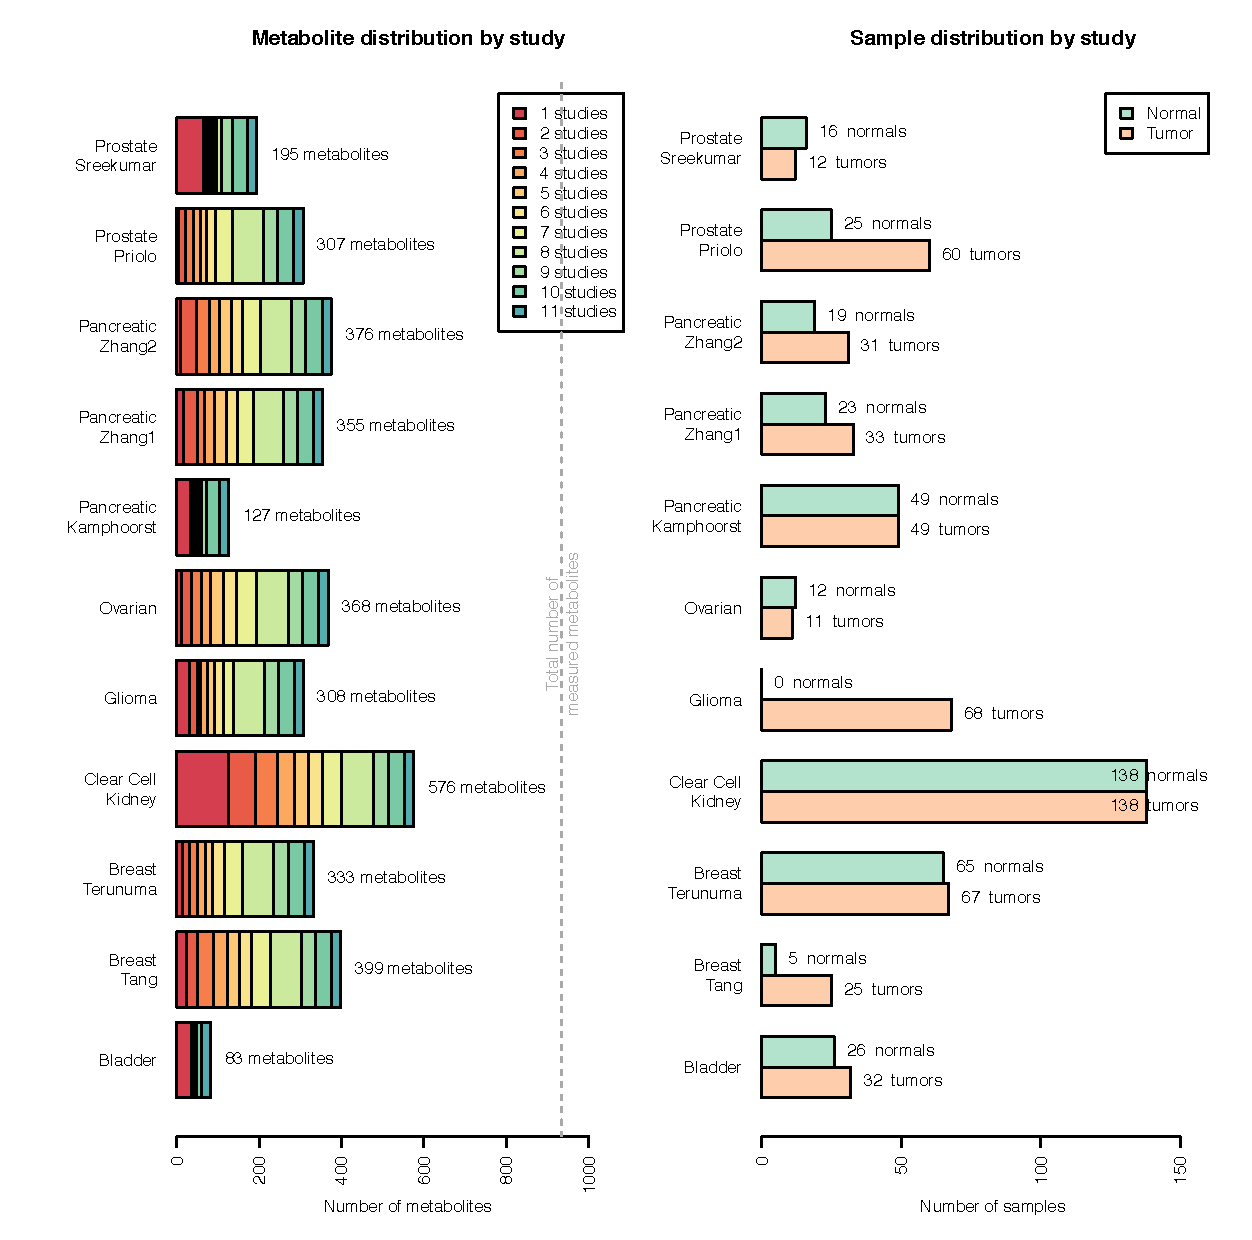
\includegraphics[scale = 0.5]{figures/Figure1/Figure1.pdf}
  \caption{Insert caption. }
     \label{fig:Fig1}
\end{figure}

\section{Assembly of a Cross-Cancer Compendium of Metabolomics Data}
We obtained published cancer tissue metabolomics data from twelve studies examining nine distinct cancer types. The goal of our study was to assemble the data from these studies into a coherent, unified dataset in which measurements of metabolites could be compared across studies. The compilation of metabolomic data was difficult for two readsons, broadly falling into the categories of data standardization and bioinformatic messiness.

A major challenge in integrating metabolomics data from multiple studies is data standardization. Data generated from mass spectrometry studies was reported as peak intensity values, which are not an absolute measure of concentration (unless there is a spiked-in reference). Therefore, data from these studies is reported as a relative quantification of a metabolite, relative to the median abundance of that metabolite across all samples in the study. As a consequence, the abundance of a metabolite $i$ in sample $j$ could only be directly compared to measurements of metabolite $i$ in other samples in the same study, but not to measurements of  (1) other metabolites in the same study, or (2) metabolite $i$ in other studies. Furthermore, due to metabolite abundances which fell outside the sensitivity of the measuring instrument, a substantial number of measurements were either missing or imputed. As depicted in Figure 1, we implemented a simple and consistent methodology for standardizing metabolite abundances for each study. 

The second major challenge was correctly identifying metabolites commonly sampled across many studies. In contrast to genes, which have a commonly accepted nomenclature, metabolites are ambiguously referred to by several names (\textit{e.g.} citrate, citric acid), and may be reported alongside an arbitrary subset of reference identifiers (\textit{e.g.} KEGG, Chebi, Pubchem, HMDB). To overcome this problem, we developed an automated pipeline to query a curated database of metabolite synonyms, based on a seed (typically, a single identifier). Then, a semi-automated script uses the expanded list of identifiers to assemble a unified metabolomic dataset (SI Data XX). Further details of the assembly process can be found in the Methods.

\begin{figure}[ht!]
  \centering
     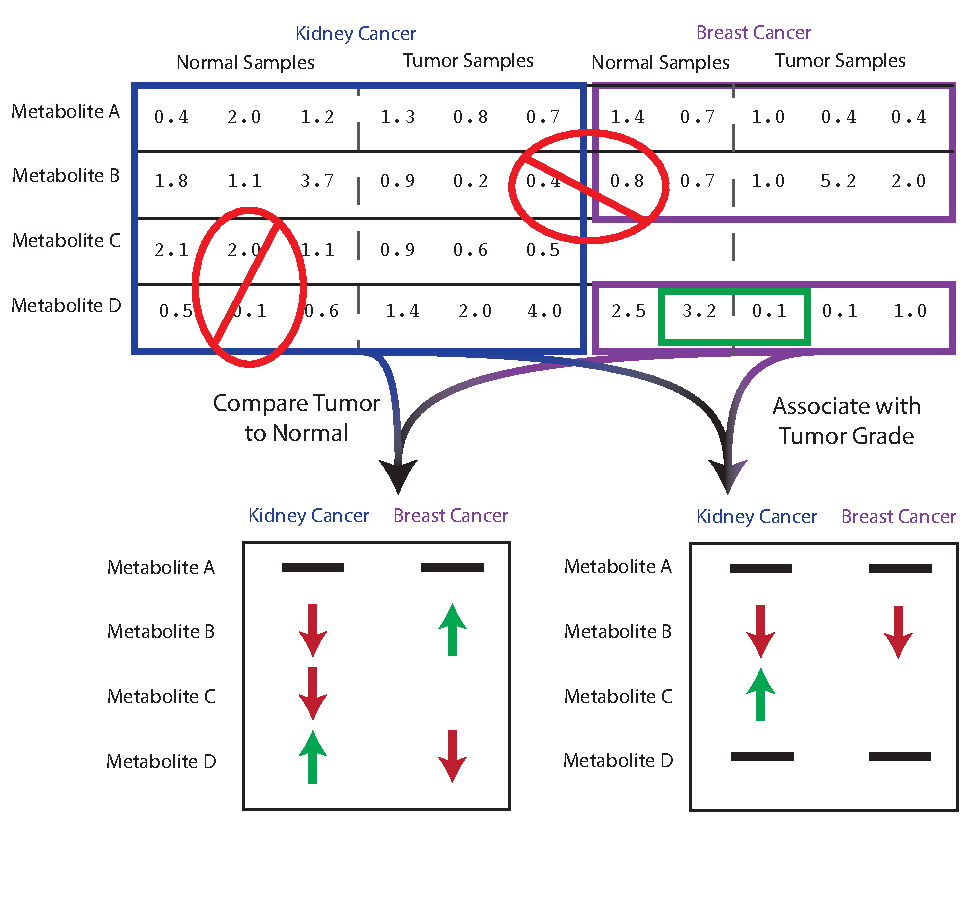
\includegraphics[scale = 0.5]{figures/Figure2/Figure2.pdf}
  \caption{Insert caption. }
     \label{fig:Fig2}
\end{figure}

\subsection{ Common Patterns of Metabolic Alterations Across Cancers}

As a first step in our analysis, we examined our assembled metabolomics data for examples of metaboites which consistently increased or decreased across a number of cancer types. To do so, we calculate the log-ratio of the mean abundance of each metabolite in a single study's tumor samples, to the mean abundance of the metabolite in normal samples. We confirmed that for the three tumor types for which we had data from multiple studies (breast, prostate, and pancreatic cancers), that metabolic changes were similar across the different studies (SI Figures XX-XX, Fisher test p-values XX breast, XX pancreatic, XX prostate).

Upon initial inspection of these results, we observed a cancer-dependent trend towards unequal proportions of metabolites which increased or decreased between tumor and normal tissues. In both breast cancer studies, we found that nearly all metabolites increased in tumor relative to normal tissue. One possible explanation for this trend was the substantial fraction of metabolites which were recurrently imputed in normal tissues because their abundance fell below the measurable sensitivity (67\% in BRCA, 37\% in BRCATang). In contrast, in all 3 pancreatic studies, we found a tendency towards an increased number of metabolites which decreased in tumors, relative to normal tissue. 

We also observed thatthe proportion of metabolites differentially abundant varied significantly from one study to the next: studies of breast and clear-cell kidney tumors found that greater than 40 percent of metabolites showed at least a 2-fold change in abundance, whereas two independent studies of prostate cancer found that fewer than 6 percent of metabolites were differentially abundant. Because the number of tumor/normal samples were comparable for these two cancer types, the differences in differential abundance were unlikely to be statistical artifacts arising from differences in sample size. This result was further confirmed by statistical boostrapping (expand here!).

We evaluated whether metabolomic changes in different studies of a common cancer type exhibited similar changes in metabolite abundnaces. Across prostate, pancreatic, and breast cancers, we observed similar differentially abundant metabolites across the studies (Fisher test, p-value XXXX).



\section{Heterogeneity in Gene Expression and Metabolite Levels}

Metabolic networks are composed of two distinct biological entities: enzymes (encoded by genes), and small molecule metabolites, which serve as substrates for these enzymes. In contrast to the limited number of studies of metabolomic changes in cancer tissues, a large number of expression studies have been published. Among these, the Cancer Genome Atlas (TCGA) consortium has reported high-resolution, publically RNA-Seq profiling of each of the tumor types described in our study. 

For each combination of KEGG pathway and metabolomics study, we calculated a differential abundance score (DA score, see Methods) for both gene expression and metabolomics data. A positive DA score indicates that the metabolites (or genes) in a pathway tend to increase in tumor samples, relative to normal tissue, while a negative DA score indicates that metabolites (or genes) tend to decrease in tumor samples, relative to normal tissue. We compared the DA scores for 92 KEGG metabolic pathways (see SI Table XX), noting a positive correlation between 

\subsection{ Warburg Effect }
The canonical observation of Otto Warburg, during his seminal studies of cancer metabolism in 19XX, was an increase in the concentration of lactate in tumor tissues. Since then, the so-called ``Warburg effect'' has been studied extensively across many systems, and has been attributed to shift away from aerobic metabolism in tumors. However, it is also well-established that mitochondrial metabolism, including both oxidative phosphorylation and other metabolic activities, is crucial to the proliferation of tumors.

We examined whether levels of lactate, a metabolic end-product of aerobic glycolysis and a commonly used surrogate for the extent of the Warburg effect in a tumor sample, were elevated in tumors compared to matched normal tissues. Surprisingly, we observed that nearly a quarter of all tumor samples investigated 

\begin{figure}[ht!]
  \centering
     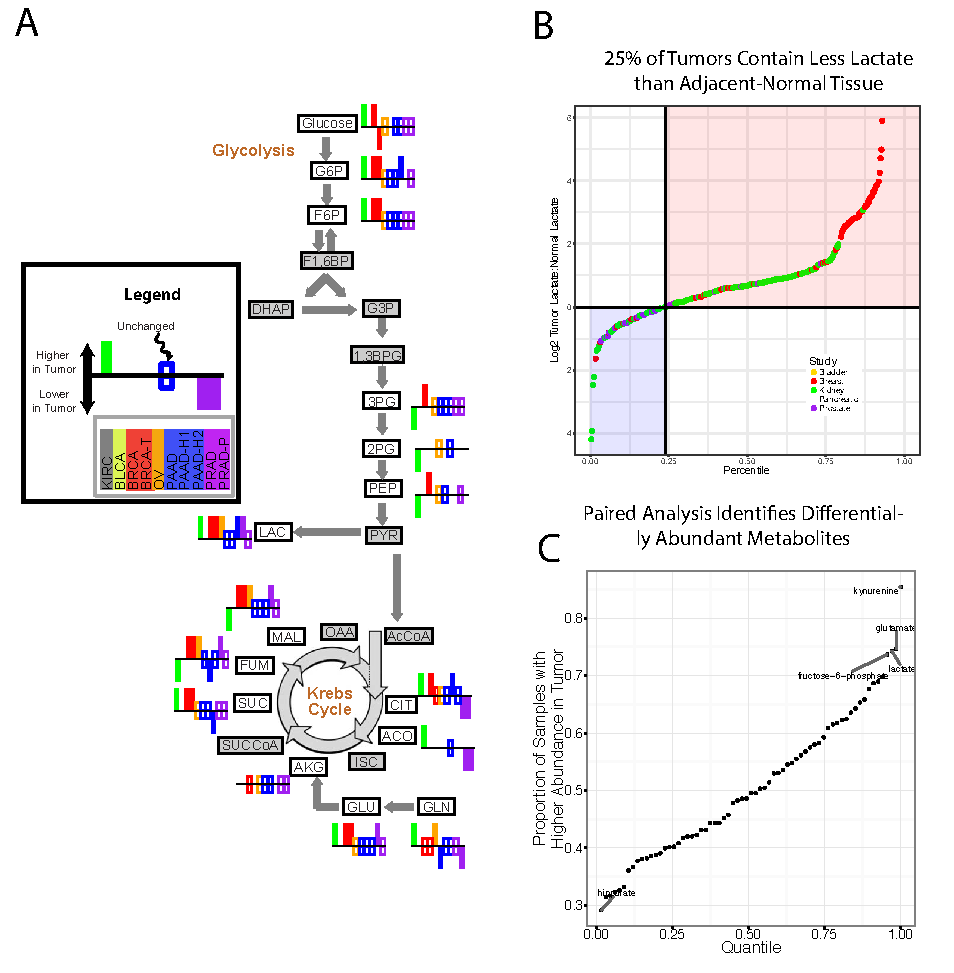
\includegraphics[scale = 0.5]{figures/Figure5/Figure5.pdf}
  \caption{Insert caption. }
     \label{fig:Fig5}
\end{figure}

\section{Discussion}

\subsection{Data Integration}
The majority of the data we collected was derived from measurements of metabolites on a relative scale. In other words, the  abundance of a metabolite was relative to other measurements of the same metabolite in the same study (\textit{i.e.} a measurement of glucose in one study could not be directly compared to a measurement of glucose in another). Furthermore, because most of the data in our analysis was derived from mass spectrometry, a substantial fraction of measurements were reported to fall below the detection threshold of the instrument. Such data is frequently reported as ``NA'' in the corresponding published data. Making this data amenable to quantitative analysis was essential for us, because it contained useful information indicating that the concentration of a metabolite was low (compared to samples where the concentration was within the quantifiable limits). Therefore, we followed prior work and applied an imputation procedure to enable use of these measurements in our analysis.We proposed a straightforward approach, based on fold change relative to matched normal tissue, to enable comparison across cancer types. 

Perhaps the first challenge we encountered during data collection was the difficulty of ``aligning'' a metabolite which had been profiled in more than one study, but was labeled with a distinct name (\textit{e.g.} lactate, lactic acid, L-lactate, (S)-lactate)). Typically, metadata regarding the chemical identity of metabolites (\textit{i.e.} KEGG IDs, PubChem IDs) was included in studies, but this metadata was universally incomplete. In most cases, a study would include either a KEGG ID or an HMDB ID for a metabolite, but not both. This made the task of finding common metabolites across studies exceptionally challenging. To overcome this challenge, we developed a bioinformatic method for assembling a list of consistent metabolite identifiers for each metabolite profiled in each study.

A second challenge arose from the large amount of incomplete data. 

Third, nearly all of the data in the meta-analysis (with the exception of the COAD/STAD data) 

The final, and perhaps most challenging, complication of our data was that, because of incomplete coverage of the metabolome, very few metabolites were profiled across more than a small number of studies. This challenge became increasingly important to address when attempting to cluster the metabolomics data across many tumor types, because the number of metabolites concordantly sampled varied from one pair of studies to the next. As a result, the dimensionality of the data varied from one pair of samples to the next, making calculating distances challenging. We proposed a non-parametric clustering approach which handled incongruous dimensionality, and showed that it identified an outlying cluster of ccRCC tumors distinguished by elevated levels of dipeptides.


\subsection{Cross-Cancer Comparison of Metabolomics Data}


\section{Methods}

\subsection{Metabolomics Data Acquisition and Normalization}
Metabolomics data from prior, published work was obtained either through the corresponding journal, or by contacting the corresponding author. The data for all studies except COAD and STAD was reported in relative abundances, \textit{i.e.} the abundance of a metabolite $i$ in sample $j$ could only be compared to other values of metabolite $i$ in different samples from the same study. For COAD and STAD, absolute abundances were reported.

Because metabolomics data does not necessarily obey a known distribution, we applied minimal normalization techniques in order to make data minimally comparable across all studies. For each metabolite in a study, we calculated the median abundance, and normalized by this abundance. Given the unknown distribution of the data in our study, we used only non-parametric statistical tests (which are independent of data distribution) to assess changes in metabolite abundance.

\subsection{Metabolic Heterogeneity}

A common obstacle in high throughput studies is the profiling of samples from different patients.

Here, we integrated expression data from the TCGA with metabolomics data from our own study. Our goal was to 
 
\end{document}
